\chapter{Lecture 30 - Laplacian in Polar Coordinates}
\label{ch:lec30}
\section{Objectives}
\begin{itemize}
\item Discuss the derivation of the Laplacian operator in polar coordinates
\item Do an example in which we solve Laplace's equation (steady-state heat equation) in polar coordinates
\end{itemize}
\setcounter{lstannotation}{0}

\section{Laplacian Operator in Polar Coordinates}

In past lectures we have used the Laplacian operator ($\nabla^2$ or $\bigtriangleup$) which is shown for rectangular coordinates below.
\begin{align*}
\nabla &= \langle \frac{\partial}{\partial x}, \frac{\partial}{\partial y}, \frac{\partial}{\partial z} \rangle \\
\nabla \cdot \nabla = \nabla^2 &= \frac{\partial^2}{\partial x^2} + \frac{\partial^2}{\partial y^2} + \frac{\partial^2}{\partial z^2} \\
&= \bigtriangleup
\end{align*}
The operator notation is convenient insofar as it is agnostic regarding coordinate system.  We can use the Laplacian in a differential equation---e.g.$\nabla^2u = 0$---without immediate regard as to whether the domain will be described in a rectangular (Cartesian) coordinate system, polar, cylindrical or spherical coordinates.  Still, at some point in time before we can hope to solve such a differential equation, we need to select a coordinate system.\marginnote[-1.5cm]{How do you pick a coordinate system?  The answer is that you select a coordinate system that makes \underline{\emph{the boundary of the domain easy to describe.}}}  Once we have done that, we need to have an expression of the Laplacian available with the appropriate independent variables.  
\begin{marginfigure}
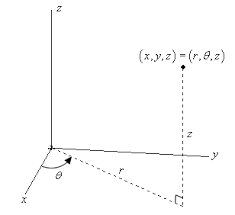
\includegraphics{lec30-cylindrical-coordinates.png}
\caption{Cylindrical coordinate system.}
\label{fig:lec30-cylindrical-coordinates}
\end{marginfigure}

\newthought{We will start} with polar coordinates.  The standard schematic of the cylindrical coordinate system is shown in Figure \ref{fig:lec30-cylindrical-coordinates}; polar coordinates are just cylindrical coordinates without the $z$-dimension.  To derive an expression for the Laplacian operator in polar coordinates, we need to be able to express the independent variables for polar coordinates---$r$ and $\theta$---in terms of the independent variables for rectangular coordinates---$x$ and $y$.  The relations between the respective coordinates are given in the margin.
\begin{margintable}
\begin{tabular}{l l l}
$r^2 = x^2 + y^2$ & & $x = r \cos{\theta} $ \\
 & \multicolumn{1}{c}{or} & \\
 $\theta = \tan^{-1}{(\sfrac{y}{x})}$ & & $y = r \sin{\theta}$\\
 \end{tabular}
\end{margintable}
So to express the Laplacian in polar coordinates, we need to express:
\begin{equation*}
u_{xx} + u_{yy} = 0
\end{equation*}
in terms of $r$ and $\theta$.  We have done changes of variables like this before; we will follow the same process.

Starting with the first derivatives, using the chain rule and product rule we have:
\begin{equation*}
\frac{\partial u}{\partial x} = \frac{\partial u}{\partial r}\frac{\partial r}{\partial x} + \frac{\partial u}{\partial \theta} \frac{\partial \theta}{\partial x}
\end{equation*}
or, using subscript notation:
\begin{equation*}
u_x = u_r r_x + u_{\theta} \theta_x
\end{equation*}
We need to replace every occurrence of $x$ with its equivalent in terms of $r$ and $\theta$. \marginnote[1.5cm]{
\noindent Here we use: 

\vspace{0.1cm}

\noindent $x = r\cos{\theta}$

\vspace{0.1cm}

\noindent and 

\vspace{0.1cm}

\noindent $(x^2 + y^2)^{-\sfrac{1}{2}} = \sfrac{1}{r}$
}
\begin{align*}
r &= \left(x^2 + y^2\right)^{\sfrac{1}{2}} \\
r_x &= 2x \frac{\left(x^2 +y^2\right)^{-\sfrac{1}{2}}}{2} \\
&= \frac{2(r \cos{\theta})}{2r} \\
&= \cos{\theta}
\end{align*}
\marginnote[1.0cm]{
Here we use the product rule and the not-so-familiar fact that:

\vspace{0.1cm}

\noindent $\frac{d}{dx}\tan^{-1}(u) = \frac{1}{1+u^2}$

\vspace{0.8cm}

\noindent $y = r\sin{\theta}$

\vspace{0.25cm}

\noindent $x^2+y^2 = r^2$

}
\begin{align*}
\theta &= \tan^{-1}(\sfrac{y}{x}) \\
\theta_x &= -\frac{y}{x^2}\left(\frac{1}{1+\sfrac{y^2}{x^2}}\right) \\
&= -\frac{y}{x^2 + y^2} \\
&= \frac{-r \sin{\theta}}{r^2} \\
&= -\frac{sin{\theta}}{r}
\end{align*}
So:
\begin{align*}
u_x &= u_r r_x + u_{\theta} \theta_x \\
u_x &= u_r \cos{\theta} - u_{\theta}\frac{\sin{\theta}}{r}
\end{align*}
Repeating the process to find the equivalent of $u_{xx}$:
\begin{align*}
u_{xx} &= \left(u_{x}\right)_{x} \\
&= \left(u_x\right)_r r_x + \left(u_x\right)_{\theta} \theta_x \\
&= \left(u_r \cos{\theta} - u_{\theta}\frac{\sin{\theta}}{r} \right)_r \cos{\theta} - \left( u_r \cos{\theta} - u_{\theta}\frac{\sin{\theta}}{r}\right)_{\theta}\frac{\sin{\theta}}{r}
\end{align*}
We would then start all over again to find $u_y$ and $u_{yy}$.  Balancing mathematical tedium with conceptual understanding, we will omit these details.  Readers are encouraged to finish the job.\sidenote{Like some other hazing rituals, deriving the Laplacian operator for polar coordinates has some (small) redeeming benefits.}

\newthought{After much tedious} work and simplification you can arrive at the expression of the Laplacian in polar coordinates given in Equation \ref{eq:laplacian-polar}.
\begin{equation}
\nabla^2u = \frac{\partial^2 u}{\partial r^2} + \frac{1}{r}\frac{\partial u}{\partial r} + \frac{1}{r^2}\frac{\partial^2 u}{\partial \theta^2}
\label{eq:laplacian-polar}
\end{equation}

We are now ready to solve Laplace's equation in polar coordinates.

\vspace{0.25cm}

\noindent\textbf{Example:} Solve the boundary value problem below based on the steady-state heat equation on a circular plate of radius $c$.

\begin{table}[h]
\begin{tabular}{l l}
$\substack{\text{Governing} \\\text{Equation}}: $& $\frac{\partial^2 u}{\partial r^2} + \frac{1}{r}\frac{\partial u}{\partial r} + \frac{1}{r^2}\frac{\partial^2 u}{\partial \theta^2}= 0, \ \ 0<r<c, \ \ 0<\theta<2 \pi $\\
& \\
$\substack{\text{Boundary} \\ \text{Conditions}}: $ & $u(c,\theta) = f(\theta), \ \ 0 < \theta< 2 \pi$\\
\end{tabular}
\end{table} 
You can confirm that the equation is linear and homogeneous.  As usual, we will use separation of variables to solve the problem.

\vspace{0.25cm}

\noindent\textbf{Step \#1:} Assume a product solution.
\begin{equation*}
u = F(r)G(\theta) 
\end{equation*}

\vspace{0.25cm}

\noindent\textbf{Step \#2:} Insert the product solution into the governing equation.  
\begin{align*}
\frac{\partial^2}{\partial r^2}(FG) + \frac{1}{r}\frac{\partial}{\partial r}(FG) + \frac{1}{r^2}\frac{\partial^2}{\partial \theta^2}(FG) &=0 \\
F_{rr}G + \frac{1}{r}F_rG + \frac{1}{r^2}FG_{\theta \theta} &= 0
\end{align*}

\vspace{0.25cm}

\noindent\textbf{Step \#3:} Separate variables.
\marginnote[2.20cm]{Note the need to multiply through by $r^2$ in order to separate terms that are a function of $r$ from those that are a function of $\theta$.}
\begin{align*}
\frac{F_{rr}G}{FG} + \frac{1}{r}\frac{F_rG}{FG} + \frac{1}{r^2}\frac{FG_{\theta \theta}}{FG} &= 0 \\
\frac{F_{rr}}{F} + \frac{1}{r}\frac{F_r}{F} + \frac{1}{r^2}\frac{G_{\theta \theta}}{G} &= 0 \\
\underbrace{\frac{r^2 F_{rr} + r F_r}{F}}_{\text{function of } r} = \underbrace{-\frac{G_{\theta \theta}}{G}}_{\substack{\text{function of} \\ \theta}} &= \lambda \\
r^2 F_{rr} + r F_{r} - \lambda F &= 0 \\
G_{\theta \theta} + \lambda G &= 0
\end{align*}

\vspace{4.0cm}

\noindent\textbf{Step \#4:} Apply boundary conditions to determine non-trivial product solution(s).  There is only one boundary condition explicitly given in this problem and it applies to the spatial variable $r$.  In this problem, however, there are some important implicit boundary conditions:
\begin{enumerate}
\item The solution must be periodic in $\theta$. This will be needed so that all the eigenfunctions in $\theta$ can be used; and
\item The solution must be finite everywhere.  In particular, it will be important that $\lim_{r\to 0} F(r) < \infty$.  
\end{enumerate}

\vspace{0.15cm}

\noindent\underline{$\lambda = 0$}
We will start with $G(\theta)$:
\begin{align*}
G_{\theta \theta} &= 0 \\
G(\theta) &= c_1 + c_2\theta
\end{align*}
Since the solution must be periodic, with period $2\pi$, $c_2 = 0$.  Consequently $G(\theta) = c_1$ is a non-trivial eigenfunction.

Checking solutions for $F(r)$:
\marginnote{ This is a Cauchy-Euler equation.  Recall from the beginning of the course that we seek solutions of the form $r^{m}$.  Inserting $r^m$ into the equation gives us: $r^2[m(m-1)r^{m-2} + mr^m]=0$ which can be simplified to: $r^m[m(m-1)+m]=0$ which is only true if $m^2 = 0$.  Recall how to deal with this double-root.}
\begin{align*}
r^2F_{rr} + rF_{r} &= 0 \\
F(r) &= c_3 + c_4 \ln{r}
\end{align*}
In order to satisfy our other implicit boundary condition, $c_4 = 0$.  So $F(r)=  c_3$ is also a valid eigenfunction.  Looking ahead, our product solution will include a constant term for the eigenvalue $\lambda = 0$.

\vspace{0.15cm}

\noindent\underline{$\lambda < 0$}: where we set $\lambda = -\nu^2, \ \nu>0$

For $G(\theta)$:
\begin{align*}
G_{\theta \theta} - \nu^2 G &= 0 \\
G(\theta) &= c_1 \cosh{\nu \theta} + c_2 \sinh{\nu \theta}
\end{align*}
Neither $\cosh{()}$ nor $\sinh{()}$ are periodic so we must conclude that $c_1 = c_2 = 0$ and that there are no non-trivial eigenfunctions for $\lambda < 0$.


\vspace{0.15cm}

\noindent\underline{$\lambda > 0$}: where we set $\lambda = \nu^2, \ \nu>0$

For $G(\theta)$:
\begin{align*}
G_{\theta \theta} + \nu^2 G &= 0 \\
G(\theta) &= c_1 \cos{\nu \theta} + c_2 \sin{\nu \theta}
\end{align*}
which is periodic, with period $2\pi$, if $\nu$ is an integer $n$.

For $F(r)$:
\begin{equation*}
r^2F_{rr} + rF_{r} - n^2F = 0 
\end{equation*}
This is a Cauchy-Euler equation.  Inserting $F = r^m$ into the equation gives us:
\begin{align*}
r^2[m(m-1)]r^{m-2} + rmr^{m-1} - n^2r^m &= 0 \\
r^m[m(m-1)+m - n^2] &= 0 \\
m^2-n^2 &= 0 \\
\Rightarrow m = \pm n, \ \ n = 1,2,3,\dots
\end{align*}
This yields the general solution: $F(r) = c_3r^n + c_4r^{-n}$.  In order to satisfy the requirement that $\lim_{r \to 0} F(r) < \infty$, we must stipulate that $c_4 = 0$.  Thus for $\lambda > 0$, the product solution is of the form:
\begin{equation*}
u_n(r,\theta) = F_n(r)G_n(\theta) = r^n\left(a_n \cos{n \theta} + b_n \sin{n \theta} \right)
\end{equation*}

\vspace{0.15cm}

\noindent Summarizing from all of the eigenvalues, the product solution is given in Equation \ref{eq:lec30-ex1-sol}.\marginnote{Be careful not to forget the eigenfunction that you found for $\lambda = 0$ which was just a constant.}

\begin{equation}
u(r,\theta) = a_0 + \sum\limits_{n=1}^{\infty} r^n \left( a_n \cos{n \theta} + b_n \sin{n \theta} \right)
\label{eq:lec30-ex1-sol}
\end{equation}

\vspace{0.25cm}

\noindent\textbf{Step \#5:} Apply the boundary condition to solve for unknown constants.  The explicit boundary condition that we have applies at $r=c$. 

\begin{align*}
u(c,\theta) = a_0 + \sum\limits_{n=1}^{\infty} c^n\left(a_n \cos{n \theta} + b_n \sin{n \theta}\right) &= f(\theta) \\
\end{align*}
On the left, we have an infinite series; on the right, we have a function that we want to represent with the infinite series.  We need to determine how to set the unknown constants $a_0$, $a_n$ and $b_n$ so that they are equal.  How do we do this?  Answer: we multiply both sides by an orthogonal function and integrate.  Our orthogonal functions are:
\begin{equation*}
\left\{1, \cos{\theta}, \cos{2 \theta}, \cos{3 \theta}, \dots, \sin{\theta}, \sin{2 \theta}, \sin{3 \theta},\dots \right\}
\end{equation*}
This set of functions is orthogonal on the domain $\theta \in [0,2\pi]$ with respect to weight function $p(x)=1$.  Carrying this out explicitly for the constant term:\sidenote{i.e. we multiply both sides by a constant---1---and integrate.  It does not matter what the value of the constant is, it is still orthogonal to all of the other eigenfunctions.}
\begin{multline*}
\int_0^{2\pi} a_0 (1) \ d\theta + \cdots \\ \sum\limits_{n=1}^{\infty} c^n \left(\cancelto{0}{ \int_0^{2\pi} a_n \cos{n \theta}(1) \ d\theta} + \cancelto{0}{\int_{0}^{2\pi} b_n \sin{n \theta}(1) \ d\theta} \right) = \int_0^{2 \pi} f(\theta) (1) \ d\theta 
\end{multline*}
so
\begin{equation*}
a_0 = \frac{1}{2\pi}\int_{0}^{2\pi} f(\theta) \ dx
\end{equation*}
Carrying out the same process using $\cos{n \theta}$ and $\sin{n \theta}$ gives us:\marginnote[1.0cm]{
Readers can confirm that: $\int_0^{2 \pi} \cos{(n \theta)}^2 \ d\theta = \pi$ and $\int_0^{2 \pi} \sin{(n \theta)}^2 \ d\theta = \pi$
}
\begin{align}
a_n = \frac{1}{c^n \pi} \int_0^{2 \pi} f(\theta) \cos{n \theta} \ d\theta \\
b_n = \frac{1}{c^n \pi} \int_0^{2 \pi} f(\theta) \sin{n \theta} \ d\theta
\end{align}

\section{MATLAB Implementation}
As usual, it is helpful to implement a solution in MATLAB so you can visualize the results.  We start by clearing out the MATLAB workspace and setting relevant parameters.

\begin{lstlisting}[name=lec30-ex1, style=myMatlab]
clear
clc
close 'all'

%% Parameters
c = 2;
N = 50;

fx_pick = 2;
%[1 | 2]
switch fx_pick
    case 1
        f = @(x) x;
    case 2
        f = @(x) ex1(x);
    otherwise
        error('Invalid case!');    
end

\end{lstlisting}

Next we implement the solution using the equations developed above.\marginnote[3.0cm]{

\ref{lst:ann30-1-1} The built-in function \lstinline[style=myMatlab]{integral()} has some name-argument pairs to customize the function behavior.  The name \lstinline[style=myMatlab]{'RelTol'} sets the \emph{relative tolerance} parameter to the value provided.  We will not go into great details here but, suffice it to say, a smaller value for \lstinline[style=myMatlab]{'RelTol'} gives a more precise result for the numeric integration.

}

\begin{lstlisting}[name=lec30-ex1,style=myMatlab]
%% solve the problem

Ao = (1./(2*pi))*integral(@(theta) f(theta),0,2*pi);

U = @(r,theta) Ao;

reltol = 1e-15;
for n = 1:N
   
    An = (1/((c.^n)*pi))*integral(@(theta) f(theta).*cos(n.*theta),...
        0,2*pi,'RelTol',reltol);   /*!\annotation{lst:ann30-1-1}!*/
    Bn = (1/((c.^n)*pi))*integral(@(theta) f(theta).*sin(n.*theta),...
        0,2*pi,'RelTol',reltol);  
   
    U = @(r,theta) U(r,theta)+ (r.^n).*(An*cos(n*theta)+Bn*sin(n*theta));
    
end
\end{lstlisting}
Having constructed a representation of the solution, we make a plot so we can see if the solution makes sense.

\begin{lstlisting}[name=lec30-ex1,style=myMatlab]
%% Make a Plot
NR = 100;
NT = 100;
R = linspace(0,c,NR);
THETA = linspace(0,2*pi,NT);
[RR,TT] = meshgrid(R,THETA);
UUp = U(RR,TT);

% plot in cartesian coordinates
XX = RR.*cos(TT); % get cartesian coordinate equivalents
YY = RR.*sin(TT);

figure(1)
surf(XX,YY,UUp,'edgecolor','none');
colormap('jet');%<-- consider alternate colormaps
c = colorbar;%<-- add a colorbar
c.Label.String = 'Temperature'; %<-- give colorbar a label
title('Lecture 30 Example','fontsize',16,'fontweight','bold');
xlabel('X','fontsize',14,'fontweight','bold');
ylabel('Y','fontsize',14,'fontweight','bold');
zlabel('U','fontsize',14,'fontweight','bold');
grid on
set(gca,'fontsize',12,'fontweight','bold');
\end{lstlisting}
The resulting plot is shown in Figure \ref{fig:lec30-ex1-plot}.  The code for the local function \lstinline[style=myMatlab]{f(x) = ex1(x)} is provided below.
\begin{marginfigure}
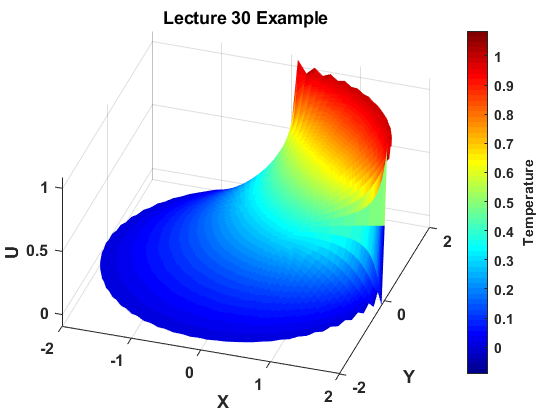
\includegraphics{Lecture_30_example.png}
\caption{Solution for the case where \lstinline[style=myMatlab]{f(x) = ex1(x)}.}
\label{fig:lec30-ex1-plot}
\end{marginfigure}
\marginnote[0.5cm]{Note the ``wiggliness'' in the solution at the points of discontinuity.}

\begin{lstlisting}[name=lec30-ex1, style=myMatlab]
%% Local functions
function y = ex1(theta)
[m,n] = size(theta);
y = nan(m,n);
for i = 1:length(theta)
    if(theta(i)>= 0) && (theta(i)< pi/2)
        y(i) = 1;
    else
        y(i) = 0;
    end
end    
end
\end{lstlisting}

